\section{Post-Merger Evolution}
\label{sec:c2_postmerger}

\begin{figure*}
\centering
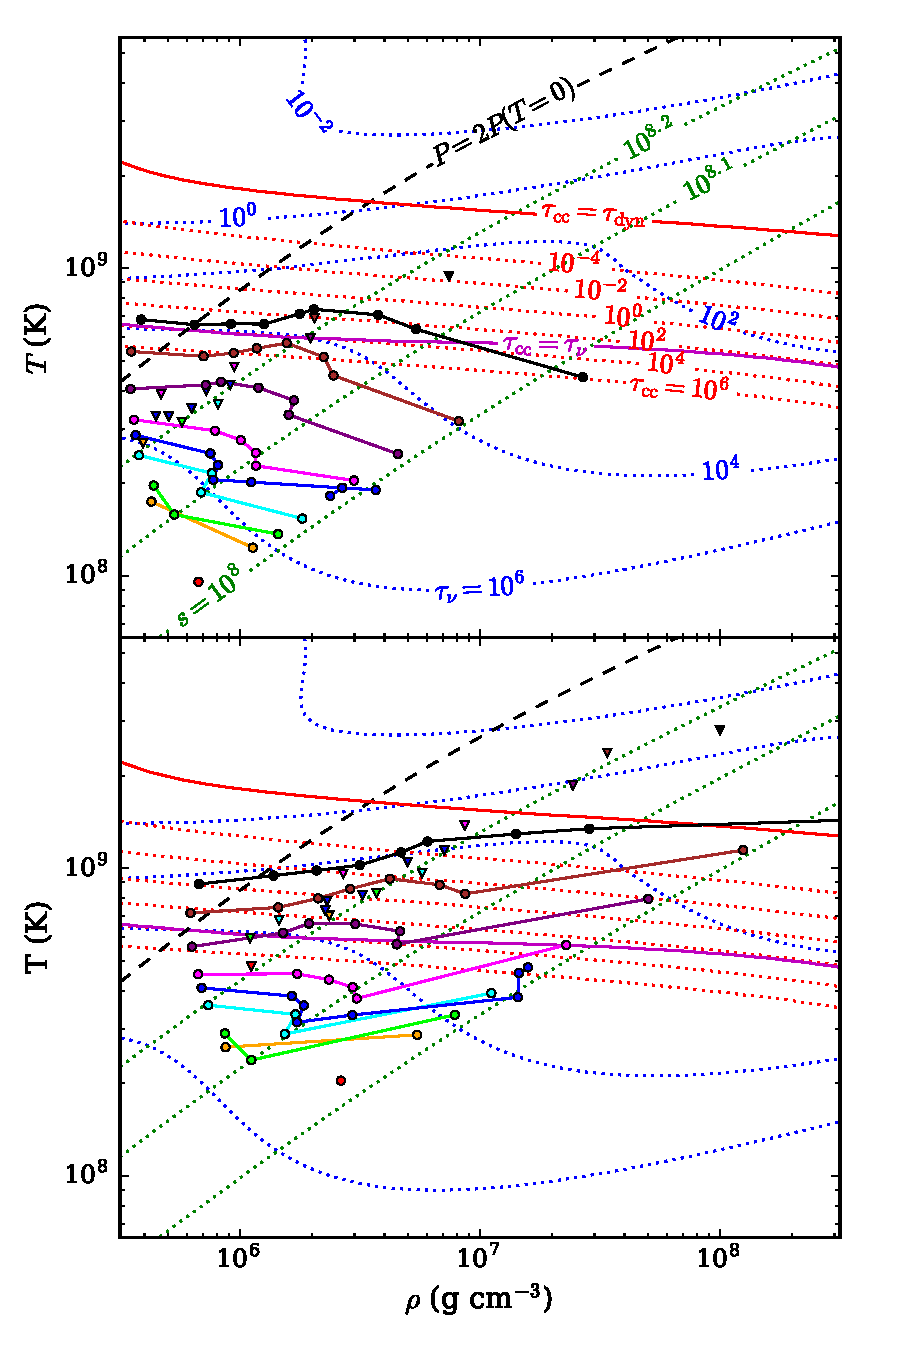
\includegraphics[angle=0,width=0.7\columnwidth]{chapter2_zhu+13/figures/Willitexplode.pdf}
\caption{Left: merger remnant maximum temperature {\Tmax} and corresponding density {\rhoTmax} for all merger remnants.  Values along the equatorial plane are marked with circles, with lines connecting points with the same accretor mass, while values along the rotational axis (only plotted for similar-mass mergers) are marked with triangles (for all, colors indicate accretor mass, encoded as in Fig.~\ref{fig:c2_constacc}).  For similar-mass mergers, equatorial temperatures have been adjusted to account for mixing in convectively unstable cores.  Right: maximum temperatures and corresponding densities following estimated post-merger evolution.  The estimate assumes that the remnant spins down completely, that all rotational energy is used to drive matter to large distances, and that the remainder adjusts adiabatically (see text).  Also shown are contours of constant neutrino cooling timescale $\tau_\mathrm{\nu}\equiv C_P T/\varepsilon_\nu$ and carbon fusion heating timescale $\tau_\mathrm{cc}\equiv C_P T/\varepsilon_{\rm CC}$, both in years, as well as entropy $S$ in ${\rm erg\,K^{-1}}$.  (Here, $C_P$ is the heat capacity at constant pressure and $\epsilon$ the specific energy loss/gain rate.)  The lines labeled $\tau_\mathrm{cc} = \tau_\mathrm{\nu}$ and $\tau_\mathrm{cc} = \tau_\mathrm{dyn}$ denote where the carbon fusion heating timescale balances the neutrino cooling and dynamical timescales, respectively.  Finally, the $P = 2P(T$=$0)$ line is shown as an approximate upper bound of the region where degeneracy pressure dominates.  All quantities were calculated using MESA \citep{paxt+11}.}
\label{fig:c2_willitexplode}
\end{figure*}

%\begin{figure}
%\centering
%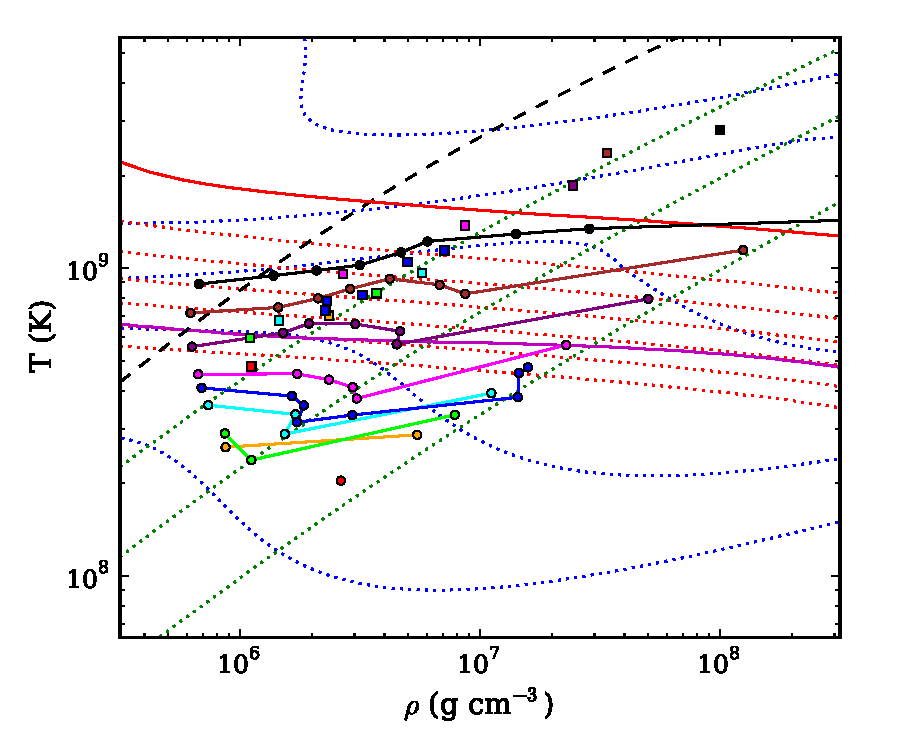
\includegraphics[angle=0,width=1.0\columnwidth]{Willitexplode2.pdf}
%\caption{As Fig. \ref{fig:willitexplode1}, except for maximum temperatures and corresponding densities following estimated post-merger evolution.  The estimate assumes that the remnant spins down completely, that all rotational energy is used to drive matter to large distances, and that the remainder adjusts adiabatically (see text).}
%\label{fig:willitexplode2}
%\end{figure}

%{\bf MHvK: CRAZY idea: for {\em all} mergers, show thin curves of $\Tmax(\phi)$; for dissimilar, this will visually look a bit like the circles, for equal, larger traces}

\begin{figure}
\centering
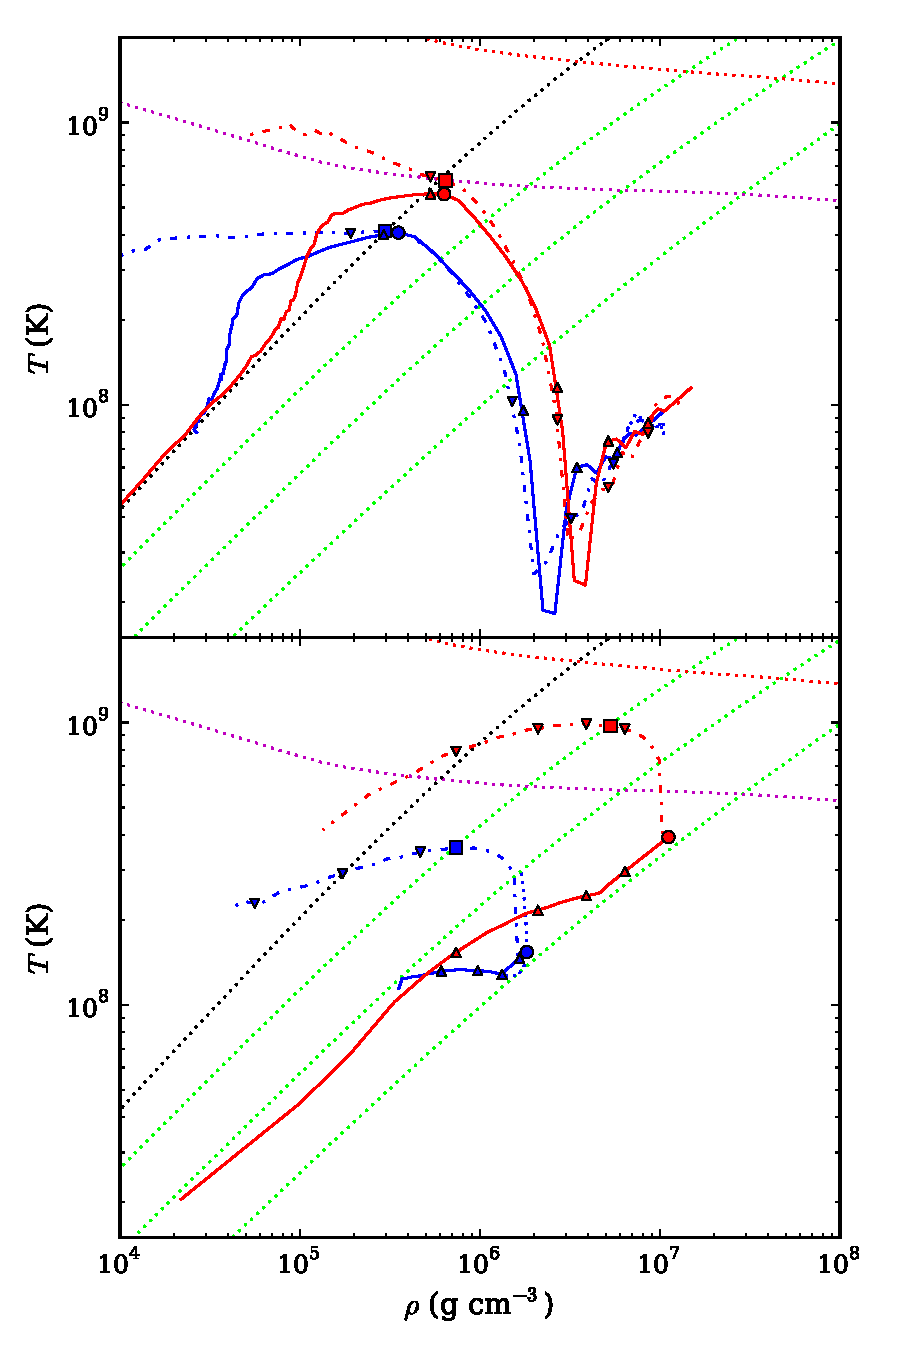
\includegraphics[angle=0,width=0.6\columnwidth]{chapter2_zhu+13/figures/PMEvolution.pdf}
\caption{Estimate of post-merger viscous evolution for 0.4 - 0.8 {\Msun} (top) and 0.6 - 0.6 {\Msun} (bottom) mergers.  In blue are shown the temperature-density structure of the merger remnant, on the equatorial plane before (dotted) and after (solid) correction for convection, as well as along the rotational axis (dot-dashed), with points marking the hottest locations (circles and squares) and steps of 0.2\,\Msun\ in spherical enclosed mass (triangles pointing up and down).  In red, estimates of the structure following viscous evolution are shown, where it is assumed that the remnant spins down completely, that all rotational energy is used to drive matter to large distances, and that the remainder adjusts adiabatically (see text).  For reference, also shown as dotted curves are the contours of constant entropy from Fig.~\ref{fig:c2_willitexplode} (green), as well as the lines where $\tau_\mathrm{cc} = \tau_\mathrm{\nu}$ (magenta), $\tau_\mathrm{cc} = \tau_\mathrm{dyn}$ (red), and $P = 2P(T$=$0)$ (black).}
\label{fig:c2_pmevolution}
\end{figure}

We now turn to the question of how our merger remnants will evolve.  To set the stage, we show in the left panel of Fig.~\ref{fig:c2_willitexplode} for all remnants the maximum temperature \Tmax\ found along the equatorial plane\footnote{The central temperatures for the 0.625 - 0.65 \Msun\ and 1.0 - 1.0 \Msun\ mergers are $\sim\!4$\% and 10\% lower than their respective maximum temperatures.  In both cases, however, the center is much denser than the off-center hotspot, and since our estimated post-merger evolution more greatly affects central material, we show the central equatorial density and temperature for these two systems in Fig. \ref{fig:c2_willitexplode} left, rather than the maximum.} as a function of the corresponding density \rhoTmax.  Here, for the similar-mass mergers for which we found convectively unstable cores (Sec.~\ref{sssec:c2_thermtrends}), we show the (lower) temperatures reached after artificially mixing them.   For those mergers, the much higher temperatures reached along the rotational axis are shown as well (triangles).  One sees the trends identified earlier: \Tmax\ is mostly set by the accretor, while \rhoTmax\ depends more strongly on the donor.  As a result, maximum temperature occurs in less degenerate conditions for dissimilar-mass mergers, crossing the degeneracy line for our most disparate cases.  One also sees that for all but the most massive accretors, carbon fusion will not start: the neutrino cooling time is shorter than the fusion heating time.  This is consistent with what was found in previous work (see Sec.~\ref{sec:c2_intro}).

\subsection{Viscous Evolution and Possible Spin Down}
\label{ssec:ch2_viscevo_possiblespindown}

Following the merger, processes that happen on timescales slower than the dynamical time can become important.  These include viscous evolution, neutrino emission, radiative or convective thermal adjustment, and magnetic dipole radiation spin-down.  Out of these, convection acts on the fastest timescale, and we already included its effect on the core in Fig.~\ref{fig:c2_willitexplode} left.  Next fastest would almost certainly be viscous evolution.  The merger remnant is unstable to both the magneto-rotational instability \citep{balbh91} and Tayler-Spruit dynamo \citep{spru02}.  Radiative adjustment is expected to be much slower, except at the surface, where radiative losses may also lead to convection in some systems \citep{shen+12,schw+12,rask+12}.  Using the standard \cite{shaks73} $\alpha$-prescription for the viscosity $\nu = \alpha c_s H$, where $c_s$ is the local soundspeed and $H$ is the scale height of the system, the viscous evolution timescale for the remnant disk is
\begin{equation}
t_\mathrm{visc} = \frac{R_\mathrm{disk}^2}{\nu} = \frac{1}{\alpha}\left(\frac{R_\mathrm{disk}}{H}\right)^2t_\mathrm{dyn} \sim \frac{10}{\alpha}t_\mathrm{dyn},
\end{equation}
implying a timescale $t_{\rm visc}\sim10^3-10^5{\rm\,s}$ for $\alpha\sim10^{-3}-10^{-1}$ and $t_\mrm{dyn} \sim 10$ s.  This is orders of magnitude smaller than both the neutrino loss timescale ($\gtrsim\!10^3$ yrs; see Fig.~\ref{fig:c2_willitexplode} left) and thermal adjustment timescale ($\gtrsim\!10^4$ yrs; \citealt{shen+12}).

It is possible that the strong differential rotation during a merger results in substantial amplification of magnetic fields.  The one known probable WD merger remnant, RE J0317$-$853, has a surface magnetic field of $3.4\times10^8\,$G \citep{bars+95,kube+10}.  If mergers lead to strongly magnetized WDs, and these WDs additionally drive an ionized outflow, the magnetic coupling between the outflow and the WD could serve to transport angular momentum out of the system, spinning down the WD.  The timescale for such a spin-down is roughly given by,
%
\begin{equation}
t_\mathrm{msd} \sim \frac{L}{\dot{M}R_A^2\Omega}
              \sim \frac{L}{(\dot M\Omega)^{3/5}(B^2R^6)^{2/5}},
\end{equation}
%
where $L$ is the angular momentum of the remnant, $\dot M$ the mass loss rate, $R_A$ the Alfv\'{e}n radius, and $\Omega$ the angular spin frequency.  For the second approximation, we used that $R_A\sim (B^2R^6/\dot M\Omega)^{1/5}$, with
$B$ the surface magnetic field and $R$ the remnant radius.  Scaling to  $B=B_810^8\,$G and $\dot M={\dot M}_{-7}10^{-7}\,\Msun{\rm\,yr^{-1}}$ (similar to what is observed for RE J0317$-$853 -- see above -- and [WR] cores of planetary nebulae [\citealt{hama97}]), and using the properties inferred for a 0.6 - 0.6 \Msun\ remnant ($L\simeq L_{\rm tot}\simeq10^{50.5}{\rm\,g\,cm^2\,s^{-1}}$, $R\simeq R_{\rm disk}\simeq10^9{\rm\,cm}$, $\Omega\simeq\Omega_{\rm max}\simeq10^{-0.3}{\rm\,s^{-1}}$, we find $t_{\rm msd}\simeq8\times10^3\,B_8^{-4/5}{\dot M}_{-7}^{-3/5}{\rm\,yr}$, which is of the same order as the neutrino cooling timescale of $\sim\!10^4{\rm\,yr}$ at the ignition line (for the whole range of remnants, $2\times10^3\lesssim t_{\rm msd}\lesssim 5\times10^4{\rm\,yr}$).

Accretion from the disk, loss of rotational support, and possible cooling of the hot envelope could all compress and heat the remnant core.  A detailed study of this is beyond the scope of this paper, but we can make first-order estimates of the effects on our merger remnants, and compare these with the more detailed analysis of \cite{schw+12} in one specific case.

For our estimates, we make four assumptions: (i) spin-down and accretion are much faster than thermal processes, and do not lead to local dissipation (i.e., particles entropies are constant in time); (ii) all angular momentum is carried away to large distances; and (iii) corresponding matter ends up with zero total energy (i.e., is at large distances and has negligible kinetic and internal energy).  From energy conservation, the last assumption implies that the remaining object will have the same total energy as our merger remnant (but a lower mass), the first that it will have the same entropy structure, and the second that it has no rotational support.  To determine the properties, we first determine the entropy profile of the merger remnant, by averaging entropy over isopotential surfaces.  We then use this entropy profile and an estimated central density to construct a spherically symmetric (non-spinning) hydrostatic model, iterating on the central density until it has the correct total energy (inside of the zero-pressure surface).  This automatically gives the mass contained in this object, which will be lower than our remnant mass, the remainder representing material that, due to dissipation of rotational energy, has expanded out to large distances and therefore provides negligible weight.  To determine the evolution of hot spots, we order remnant particles by potential, and map them to their new positions in the final object, calculating new temperatures from the new densities, again assuming their entropy did not change (entropy is not constant over isopotential surfaces, so these temperatures are not strictly consistent with the hydrostatic model).

In Fig.~\ref{fig:c2_pmevolution}, we show the results of our evolutionary estimate for our fiducial 0.4 - 0.8 and 0.6 - 0.6 {\Msun} systems.  For the former case, the core-envelope, originally 0.90\,\Msun, accretes 0.06\,\Msun\ from the disk, the remaining 0.25\,\Msun\ going to large distances.  The central core is not significantly heated, while the lower-density hot envelope is, with the outer hot envelope along the rotational axis passing the ignition line.  Since this material is almost non-degenerate, the resulting nuclear burning will likely be stable, or be extinguished by expansion.  Thus, not unexpectedly, the hot envelopes of dissimilar-mass mergers are not good candidates for a nuclear runaway.  

%MHvK: I removed: As loss of rotational support should result in compression mainly along the equatorial plane, much of the rotational axis hot envelope may instead remain unperturbed, or be squeezed out to larger distances and adiabatically cool.

For the 0.6 - 0.6 {\Msun} system, the center of the final, spun-down object is at much higher density and temperature than the remnant, while much of the outer regions have become less dense and cool.  The latter happens because similar-mass mergers have strong rotational support, and if this is removed their binding energy increases significantly.  To compensate for this, a large amount of mass has to expand to large distances, causing the core-envelope mass to decrease from 1.11 {\Msun} to 0.91 {\Msun}.  In the final object, the hottest point on the equatorial plane does not reach the ignition line, but the significantly hotter points above and below the equatorial plane do, at densities under which degeneracy pressure still dominates.  Hence, if the hot spots indeed compress with the rest of the remnant, a nuclear runaway could be triggered.  (Of course, a nuclear runaway would start as soon as the heating timescale becomes shorter than the compression timescale, which may happen closer to the ignition line.)

%MHvK: removed the sentence below since we do not really know the timescale; see added sentence above.  I also think we should remove the yellow line (perhaps instead include some heating timescale lines)
%The assumptions for our estimate break down for any degenerate points in the remnant that reach past the yellow $\tau_\mathrm{cc} = 10^{-4}$ yr curve: at this point the nuclear burning timescale becomes smaller than the viscous evolution timescale, and it becomes important to consider nuclear energy generation in addition to accretion, but at this point a nuclear runaway has occurred.

In the right panel of Fig.~\ref{fig:c2_willitexplode}, we show the results of applying our estimates to all our merger remnants.  One sees that all compress and heat, and almost every remnant whose accretor mass is above 0.8\,\Msun\ will reach ignition somewhere on the equatorial plane, in many cases under degenerate conditions.  We also chart the evolution of the off-center hot spots in similar-mass mergers (square points), and while they are at lower density, they remain degenerate and are all pushed substantially further above the ignition line than their counterparts on the equatorial plane.  Almost all similar-mass mergers with an accretor mass above 0.5 {\Msun} could therefore experience nuclear runaways due to their hot spots, though at least some of them will become non-degenerate before an explosion can occur.

The above suggests it is at least plausible that many of our mergers would eventually ignite in degenerate conditions, and that it thus is worthwhile to simulate their evolution in detail.  Suitable simulations have recently been pioneered by \cite{shen+12} and \cite{schw+12}.  \citeauthor{shen+12} started with a one-dimensional simulation, where they ported the remnant of a 0.6 - 0.9 {\Msun} merger (from \citealt{dan+11}), and evolved it assuming a $\gamma = 5/3$ polytropic equation of state and an $\alpha = 10^{-2}$ viscosity.  They find the system spins down completely due to outward angular momentum transport, and the rotationally-supported thick disk is transformed into a tenuous, thermally-supported envelope that hardly affects the core.  Over longer, thermal evolution timescales (simulated using MESA, \citealt{paxt+11}), this tenuous hot envelope cools, compresses the core, and lights off-center convective carbon burning, eventually turning the remnant into an ONe WD (that may end its life in an accretion induced collapse).

\cite{schw+12} went a step further, porting the same 0.6 - 0.9 {\Msun} simulation, as well as seven other systems, into two-dimensional ZEUS-MP2 simulations \citep{haye+06}, using the Helmholtz equation of state and an $\alpha=3\times10^{-2}$ viscosity.  They confirm the one-dimensional results, finding complete spin-down and transformation of the rotationally supported disk into a tenuous, spherically symmetric, hot envelope.  They find a 50\% increase in the temperature of the hottest point, and a factor of 3 increase in the corresponding density.  They also find entropy to roughly be constant in the remnant, except in the outer regions and at the very center, where dissipation of rotational energy leads to heating.

It is encouraging that the results of the above detailed simulations are similar to what we find using our first-order estimates.  For our 0.6 - 0.9 {\Msun} remnant, our estimate give increases for the hottest equatorial point of a factor of 2.5 in density and 1.6 in temperature, reasonably close to what is found by \citeauthor{schw+12}\footnote{For the hottest point along the rotational axis, we find a factor of 4.8 increase in density and 2.1 increase in temperature, suggesting our model does not depict as well the evolution of the outer hot envelope along the rotational axis.}.  Thus, our simplifying assumptions appear to be appropriate at least for dissimilar-mass mergers, where most of the rotational dissipation will be in the disk and envelope, and the structure of the remainder is roughly spherically symmetric (both in density and temperature).  It is not clear our estimates would be equally good for similar-mass mergers, where rotational dissipation should occur throughout the star, heating the entire remnant, and where there are substantial differences between the remnant's density and temperature structures.  In particular, the rotational axis hotspots may dissipate, which would potentially make it more difficult for a similar-mass system to achieve a runaway.  It will thus be particularly interesting to simulate the further evolution of those remnants in more detail.  Unfortunately, no such remnants were included by \citeauthor{shen+12} and \citeauthor{schw+12}.

\subsection{Possible Explosions?}

From our estimates, it seems that, as suggested by \citeal{vkercj10}, many merger remnants will ignite carbon fusion.  If a detonation is triggered, the resulting explosion may well resemble an SN Ia.  Indeed, if the remnants spun down before ignition, their structures are sufficiently close to that of a cold WD that the calculations of \cite{sim+10} should apply.  From our estimates, for mergers that have a total mass between 1.2 and 1.4\,\Msun\ (which should be the most common ones), the final objects have masses between $\sim\!0.9$ and $\sim\!1.1$ \Msun\, which matches fairly nicely the range of $\sim\!1$ to $\sim\!1.2$ \Msun\ required to reproduce the observed range of SN Ia luminosities \citep{sim+10}.

%MHvK: I think this is a bit too much detail, where we  add relatively little; replaced by a single sentence above

Of course, it is far from clear whether ignition leads to a detonation, since we do not currently understand how detonations are triggered (\citealt{seit+09,woos+11}, and references therein).  Generally, it should help that ignition in our remnants is at much lower density (a few $10^7\,{\rm\,g\,cm^{-3}}$) than is the case for near-Chandrasekhar models ($\sim\!10^9{\rm\,g\,cm^{-3}}$), because complete burning leads to much larger relative overpressures (e.g. \citealt{mazumw77}; \citealt{seit+09}).  Also, if a deflagration is started, plausible mechanisms to transition to a detonation all seem to require densities around $10^7\,{\rm\,g\,cm^{-3}}$, where the conductive flame speeds are slower and the separation between the various burning fronts increases (e.g., \citealt{woos+09,woos+11}).

An interesting aspect of our results is that for all cases ignition likely happens off-center: in shells for dissimilar-mass mergers and in hot spots along the rotational axis for similar-mass ones.  Previous one-dimensional simulations suggested off-center ignition would lead to a slow deflagration flame that turns the CO WD into a ONe WD (e.g., \citealt{saion85}).  However, these calculations assumed a hot spot many pressure scale heights above the center.  For ignition closer to the center, a deflagration plume is produced (e.g., \citealt{aspd+11}), which may transition to a detonation \citep{seitcr11} and unbind the star.   

Given our findings, it seems likely that, if a detonation occurs, it will be triggered off-center.  It would be interesting to simulate the resulting explosion, and see whether one could reproduce the observational evidence for asymmetries, which have been interpreted in terms of off-center ignition (though so far only in the context of near-Chandrasekhar models; \citealt{maed+10a,maed+10b}).

Finally, while we simulated only mergers of CO WDs, we can extrapolate our results to more massive ONe WDs.  For these, the temperatures would be at least as high as for our 1\,\Msun\ accretors, and, after further viscous evolution, the mergers should become hot enough to ignite Ne burning.  If this also leads to a detonation, the lower fusion energy released would likely lead to a less energetic explosion than expected for a CO WD merger, but it would produce far more $^{56}$Ni and have a very large mass.  Plausibly, it would resemble an SN Ia like SN 2009dc, which had unusually low ejecta velocities, produced $\sim\!1.8\,\Msun$ of $^{56}$Ni and had a total ejecta mass of $\sim\!2.8\,\Msun$ \citep{taub+09}.

%\subsection{Future Work}

%In Sec. \ref{ssec:initcond} we noted that we use approximate initial conditions, and it has been shown \citep{dan+12} that accurate initial conditions non-negligibly affect the structure of the merger remnant.  As discussed in Sec. \ref{ssec:varyingazero}, to first order we expect the extended period of quasi-stable mass transfer found in initial condition studies would result in more mergers across our parameter space resembling dissimilar mass mergers, since at final coalescence the donor would have become less massive, and the accretor more.  This could reduce the number of systems in our parameter space study that would resemble similar mass mergers, particularly if more than $\sim0.1$ {\Msun} is generally transferred before coalescence.  If the amount of mass transferred depends on total system mass (rather than just {\qrho}), then the homologies we presented in Sec. \ref{ssec:samplingofmergers} would also be affected.  No study of how accurate initial conditions for unsynchronized systems has thus far been published.  We are in the process of generating accurate initial conditions for our unsynchronized systems in order to quantify how the trends we have found would be affected.

%The structure of the remnant is affected by whether or not the merging binary was synchronized, a still-unresolved issue (Sec. \ref{ssec:compwithothers} \emph{PERHAPS WE SHOULD MOVE THAT ENTIRE DISCUSSION HERE, SINCE WE DON'T COMPARE WITH ANYONE EXCEPT LOREIG ANYMORE??}).  Perhaps the most effective way of investigating this issue is with observation.  Two very short (period on the order of minutes) binary systems are known to be eclipsing \citep{stei+10,brow+11}, allowing in principle measurement of the rotational velocity modulo the inclination to the observer (which may be different than the inclination of the orbital plane), $v\sin i$, of both stars through the Rossiter-McLaughlin effect.  Rotation could also be measured through the broadening in the narrow, non-LTE core of H$\alpha$.  We are currently performing such measurements on SDSS J065133.33+284423.3, in order to compare with theoretical tidal dissipation models.

%To determine the fate of our merger remnants, we must simulate the post merger evolution of our parameter space.  \citeauthor{schw+12} have already demonstrated the effectiveness of 2.5D grid-based simulations in realistically describing this evolution.  We are currently preparing to port our remnants into a code similar to that of \citeauthor{schw+12}'s, in order to extend their work by filling out the parameter space of CO WD mergers.  Most critically, we will simulate the evolution of similar mass mergers, which is missing from \citeauthor{schw+12}.  The entire structure of an similar mass merger remnant would be affected by spin-down (only the outer envelope is greatly affected for dissimilar mass mergers), and our estimates above indicated that these systems are most likely to experience a core nuclear runaway when compressed.

%Ultimately, the physical robustness of \citeal{vkercj10}'s SN Ia channel also depends on whether or not, even if a detonation can be triggered in an evolved remnant (Sec. \ref{ssec:postmerger}), the resulting explosion can reproduce observationally established properties of SNe Ia.  \cite{sim+10}'s are of bare, cold sub-{\Mch} WDs.  True merger remnants feature material in extended tenuous envelopes, and possibly outflows.  If the remnant core produced an SN Ia, the explosion ejecta will shock heat this material, changing the early-time light curve of the SN Ia \citep{frye+10}.  Because they are insufficiently dense and are thought not to have an extended deflagration phase before detonating, sub-{\Mch} objects also cannot produce stable $^{58}$Ni from electron capture during the explosion.  $^{22}$Ne pollution from burning of CNO cycle catalysts, however, can result in stable nickel production in the pure detonation of sub-{\Mch} WDs, though the amount generated, and the signature imprinted in the SN Ia's spectra, will differ from those of electron capture.  Since [Ni II] lines are indeed seen in the late-time spectra of SNe Ia \citep{gera+07, maed+10a}, it is not yet obvious which stable nickel generating method is more favored by observations (see discussion in \citealt{vker12}).  These questions remain to be investigated with regard to \citeal{vkercj10}'s channel.

%Stable, relatively slow moving $^{58}$Ni has been sighted in late-time SNe Ia spectra (ex. \citealt{gera+07}).  $^{58}$Ni can be generated either through electron capture during nuclear burning in high-density material, or by burning $^{22}$Ne.  While $^{22}$Ne is expected to gravitationally settle to the center of single WDs, it will re-mix during a merger, and in \citeal{vkercj10}'s channel there is insufficient time for it to settle before an explosive nuclear runaway occurs.  This means that, if an SN Ia occurs, the $^{22}$Ne distribution generated by the merger will determine where $^{58}$Ni is generated during the explosion.  There is therefore the potential for spectroscopic features distinguishing explosions due to \citealt{vkercj10}'s SN Ia channel from those due to other channels.  We are currently exploring the fate of the He atmosphere and Ne pollutants using tracer particles in our simulations.

\section{Conclusion}

We have performed a large, detailed parameter-space study of CO WD mergers, extracting pertinent properties and profiles for each remnant, and studying how these vary across parameter space.  For a merger involving dissimilar-mass WDs, with low {\qrho} = {\rhocrat}, the outcome is a cold, slowly rotating, degeneracy-supported remnant core, which is essentially unaffected by the merger, surrounded by a hot, roughly spherical envelope and, further out, by a sub-Keplerian disk.  For a similar-mass merger, with high {\qrho}, an ellipsoidal core is produced along with a small disk, and the entire remnant is hot and partly supported by rotation.  The transition between these two regimes is smooth, but occurs roughly at $\qrho\simeq0.6$, or equivalently a mass difference $\Delta M= \Ma-\Md \simeq 0.1$.  We found that for a fixed {\qrho}, merger remnant curves are roughly homologous.  We also presented trends for a number of merger remnant properties, providing linear scaling relations and best fits for most of them, hoping these can guide theoretical understanding and help analytical estimates.

We made first-order estimates of the post-merger viscous evolution and spindown, and found that it is plausible that a large fraction of the mergers simulated will eventually experience a nuclear runaway, as was suggested by \citeal{vkercj10}, and thus possibly end as thermonuclear supernovae.  Further, detailed, simulations of this evolution across the whole parameter space, using techniques similar to those of \citet{shen+12} and \citet{schw+12}, would be required to confirm this.  If the evolution of these remnants results in a detonation, a detailed comparison of the resulting light curve with observations must be carried out.

Our work represents one of the most detailed parameter studies of WD mergers to date.  It would benefit, however, from resolution of a number of topics.  First, for greater precision, it will be necessary to use better initial conditions.  For synchronized systems, it is already known this has nontrivial effect on the outcome \citep{dan+11,dan+12}, and our results suggest it is important also for non-synchronized systems.  Unfortunately, for the non-synchronized case, it is not trivial to implement the initial conditions, but better approximations are possible.  Second, it would be useful to try to compare with merger simulations done with a grid code, which should have become more straightforward now that good moving mesh codes have become available \citep{spri10,duffm11}.  More generally, whether or not WDs are synchronized before the merger remains unknown, yet clearly affects the resulting merger.  Hopefully, this can be resolved empirically, by measuring the spin frequency for WDs in the very short-period binaries that have recently been discovered (e.g., \citealt{brow+11}).

We thank Pablo Lor\'{e}n-Aguilar, Enrique Garc\'{i}a-Berro, Stuart Sim, Enrico Ramirez-Ruiz, Marius Dan, James Guillochon, Evan Scannapieco, Cody Raskin and Ken Shen for insight into their simulations and useful discussion on the physics of mergers and post-merger evolution.  We are grateful to Frank Timmes for creating the Helmholtz equation of state, and assisting us with its implementation in Gasoline, as well as to Bill Paxton and the MESA team for creating MESA and making it modular.  This work made extensive use of NASA's ADS and was supported by the Vanier and Discovery grants of Canada's Natural Sciences and Engineering Research Council (NSERC).
